\chapter{Framework Modules}
\section{Module: Core-Framework}
\label{sec:core}
\subsection{Network}
- explain leecher, seeder, peer, core concepts etc


\subsubsection{Automatic Connect}
\label{subsubsec:autoconnect}

Every peer can be both a leecher and a seeder. While every leecher has to manually connect to a seeder for the first time, after this a leecher is able to automatically connect to other seeders. This is because every leecher who is paired with a seeder announces the address of its seeder to all seeders it is connected with. The figure \ref{fig:autoconnect} show this in detail.

\begin{figure}[b]
\centering
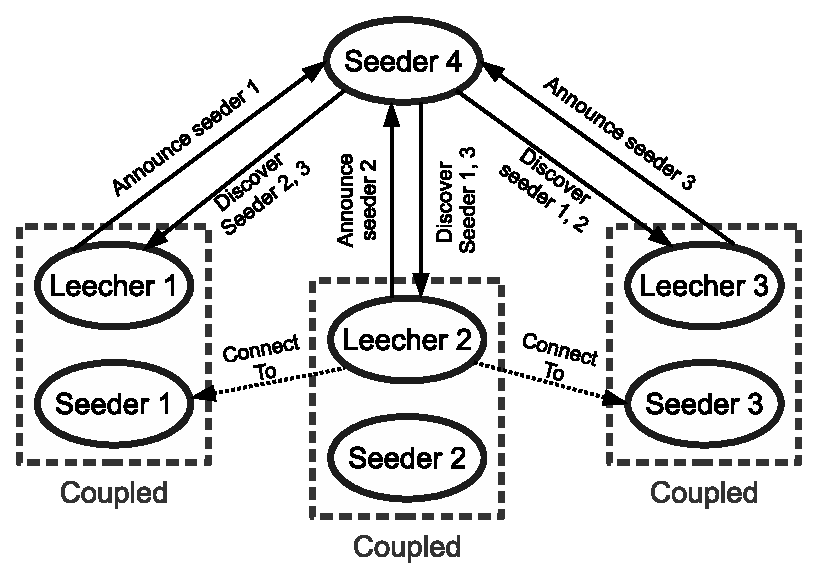
\includegraphics[width=8cm]{autoconnect}
\caption{Seeder Discovery}
\label{fig:autoconnect}
\end{figure}

\pagebreak

Here Leecher 1, 2 and 3 announce the address of Seeder 1, 2 and 3 respectively to the initial Seeder. The initial seeder then broadcasts those addresses to all connected leechers. This way the leechers get to know each and can connect to the remaining seeders. Though in figure\ref{fig:autoconnect} only Leecher 2 is illustrated, Leecher 1 and 3 connect to the remaining seeders, too. Of course this works recursively, so if one of the remaining seeders already has other leechers connected to it those will also be found. So in the end the topology is just a mesh with $n^2$ connections where $n$ refers to the total number of peers where every leecher of each peer is connected to every seeder of all other peers. The figure \ref{fig:mesh} show this from the point of view of Leecher 1 from Peer 1 assuming there are 7 other peers.

\begin{figure}[ht]
\centering
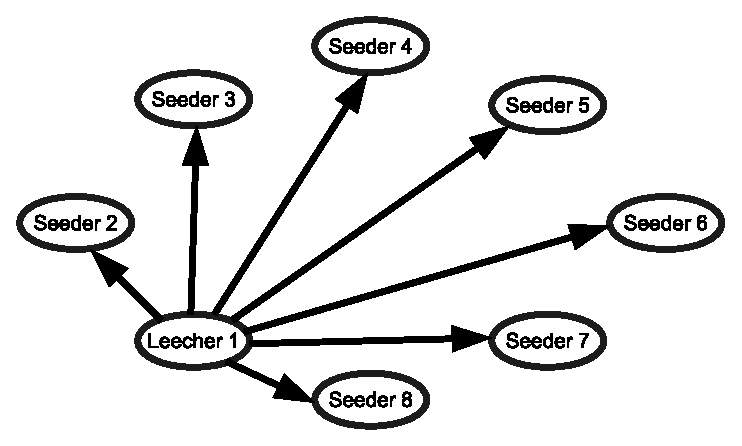
\includegraphics[width=8cm]{mesh}
\caption{Mesh topology}
\label{fig:mesh}
\end{figure}

While this topology is really great in terms of knowledge where every peer knows exactly what data sets the other peers have and thus can download data efficiently, it is also quite expensive and would not scale indefinitely. To improve scalability and reduce efficiency the number of connections per peer can be limited which limits the knowledge of each peer and thus the ability to make good decisions what to download from whom. This is explained later in section \ref{sec:benchmark} in more detail.

If a connection for what ever reason terminates the framework is able to reconnect if the peer is still online. This will be detected by periodic address broadcasts of each seeder. So if for instance Peer 1 lost the connection to Peer 2 but both Peers are still connected to Peer 3 then Peer 3 will notify both that each peer still exist.

\subsubsection{Meta-Data Announcements}

After a Leecher connects to a Seeder the Leecher does not know anything about the Seeder. As previously explained in section \ref{subsubsec:autoconnect} the Leecher discovers new Seeders through the Seeders it is currently connected to. The way the Leecher gets knowlege about what data sets a Seeder offers works a similiar way. A Seeder announces to all connected Leechers periodically what data sets it has to offer. It basically transfers a list of Meta-Data, which is explained further in section \ref{subsubsec:metadata}, so that every Leecher can update its knowledge about the Seeder. 

As an optimization the Seeder only transfers new Meta-Data. So if a data set does not change at all, a Seeder will never transfer a second announcement of this data set. Another optimization is that while a Leecher downloads a chunk from a Seeder, the Seeder will also not transfer any announcements during this period, which is explained further in the next section \ref{subsubsec:downloadreq}.

\subsubsection{Download Requests}
\label{subsubsec:downloadreq}



\subsubsection{Nonblocking I/O}
\subsubsection{Transport: Local}
\subsubsection{Transport: TCP}
\subsection{Concurrency}
\subsubsection{Event-Loop}
\subsubsection{Lock-Free-Progamming}
\section{Module: DataBase}
\label{sec:database}

The DataBase Module represents a generic interface for any kind of data. While the Core-Framework transfers data between peers the data has to be read from and written to some kind of storage. This storage has the responsibility to verify incoming data in terms of consistency and validation. But to do so the storage has to know about the structure of the data. Because of that the metadata which describes a given data set is stored together with the data as key-value pairs.

\subsubsection{Meta-Data}
\label{subsubsec:metadata}

The Meta-Data contains information about a given data set. Those information are:
\begin{itemize} 
\item Name
\item Description
\item ID
\item Size
\item Chunks
\item Hash
\item ChunkHashes
\end{itemize}
The Name and Description fields are used for human-related tasks. The ID has to be globally unique and is used for streaming purposes which will be explained later. The Size field determines the total size of the data set including all chunks which leads to the next field. The Chunks field is a bit set which simply stores one or zero bits for existing or missing chunks respectively. The length of the bit set determins the number of chunks a data set has. The Hash field contains a check sum generated by a strong hash algorithm like SHA from the whole data set. The ChunkHashes field does the same but for each chunk individually. This way the storage can verify single chunks as well as the data set in total. The reason why there is an extra Hash field for the whole data set is to reduce the chance of hash collision. Two data sets are equal if all of their fields are also equal.

\subsubsection{Virtual}
\subsubsection{Filesystem}


\section{Module: Algorithm}
\label{sec:algorithm}

\section{Module: Monitoring}
\label{sec:monitoring}

